\part{Analysis}
\textit{Results from the implementation}

\chapter{Results}

The HDR-NN training implementations were benchmarked on the iMX6SDB evaluation board. Model accuracy, execution time and peak memory utilised during the training of the model is compared while varying the number of layers and the neurons in each layer

\section{HDRNN comparisons}
\begin{itemize}
	\item \textit{State the reasoning behind comparisons of HDRNN implementations - e.g same accuracy when initialised with the same random weights \dots}
	\item \textit{Describe the performance measure considered - execution times, network accuracy, power usage \dots motivated in Theory chapter}

\end{itemize}

\subsection[Python - Numpy]{Python Numpy based HDRNN}
\textit{Performance of textbook HDRNN using Python \& Numpy}

\begin{center}
	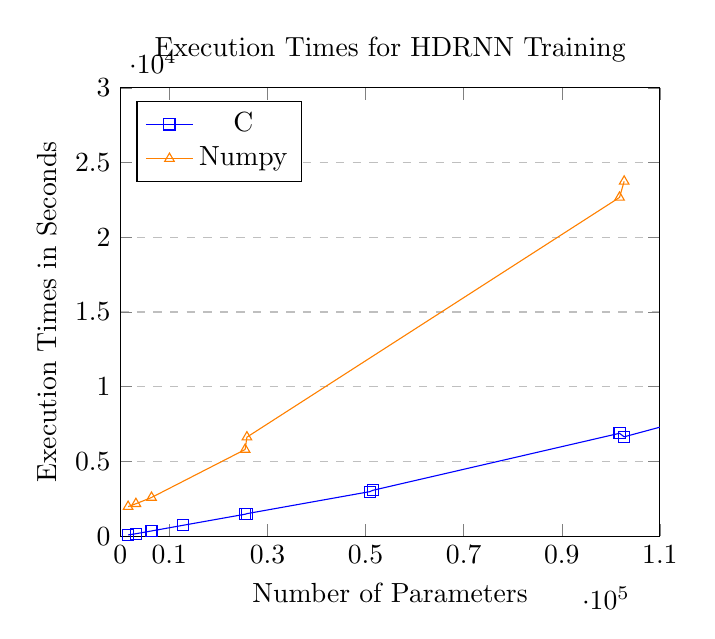
\begin{tikzpicture}
		\begin{axis}[
			title={Execution Times for HDRNN Training},
			xlabel={Number of Parameters},
			ylabel={Execution Times in Seconds},
			xmin=0, xmax=110000,
			ymin=0, ymax=30000,
			xtick={0,10000,30000,50000,70000,90000,110000},
			ytick={0,5000,10000,15000,20000,25000,30000},
			legend pos=north west,
			ymajorgrids=true,
			grid style=dashed,
		]

		\addplot[
			color=blue,
			mark=square,
			]
			coordinates {
				(1600,85)
				(3190,164)
				(6370,351)
				(12730,725)
				(25450,1470)
				(25818,1509)
				(50890,2983)
				(51450,3068)
				(101770,6885)
				(102714,6650)
				(203530,15581)
			};


		\addplot[
			color=orange,
			mark=triangle,
			]
			coordinates {
				(1600,1978)
				(3190,2171)
				(6370,2589)
				(25450,5799)
				(25818,6628)
				(101770,22670)
				(102714,23744)
			};
			\legend{C, Numpy}

		\end{axis}
	\end{tikzpicture}
\end{center}
The training time was recorded for hidden layer sizes of 2, 8, 32, and 128 and 
found that it increases exponentially with the number of parameters. This is due to 
the fact that the amount of calculation in a fully connected network increases with the 
number of neurons, leading to longer training times. 
Further, when the number of 
neurons in a single layer exceeds 32, the accuracy of the model is observed to decrease 
due to overfitting. To improve accuracy, adding another layer with 16 neurons is found to 
be beneficial without significantly increasing the time required for computation. 
In fact, for larger network sizes, it is observed to even reduce the computation time required. 
Regardless of the hidden layer sizes, the peak memory utilisation remains constant because the 
peak usage occurs when \dots  

\subsection[Tensorflow Lite]{Tensorflow-Lite based HDRNN}
\textit{Performance of a similar network on Tensorflow lite}

\subsection[C]{C based HDRNN}
\textit{Performance of a similar network written in C}


\subsection[CPP - Eigen]{CPP based HDRNN}
\textit{Performance of a similar network written in CPP}

\section{CMSIS-NN based Optmisations}
\textit{Further breakdown of the performance achieved from different optimisation techniques}

\subsection{Quantisation}
\textit{future: Training Network with Quantized weights}

\subsection{Pruning the Network}
\textit{future}

\chapter{Discussion}
\begin{itemize}
	\item \textit{Contrast development process for the ML programming paradigms}
	\item \textit{Which optimisation approaches gave the most in improvement?}
\end{itemize}

\chapter{Conclusion and Future Work}
\textit{What does it all mean? Where do we go from here?}
